\documentclass[11pt,a4paper]{article}
\usepackage[margin=1in]{geometry}
\usepackage[T1]{fontenc}
\usepackage[utf8]{inputenc}
\usepackage{lmodern}
\usepackage{booktabs}
\usepackage{graphicx}
\usepackage{float}
\usepackage{amsmath}
\usepackage{hyperref}
\hypersetup{colorlinks=true,linkcolor=blue,urlcolor=blue,citecolor=blue}

\title{Predictive Sales Analytics Engine\\\large Leakage-Safe Phase-1 Repeat-Purchase Prediction}
\author{Aditya Kammati}
\date{March 22, 2026}

\begin{document}
\maketitle

\begin{abstract}
This project builds a leakage-safe phase-1 predictive sales analytics pipeline on the Olist Brazilian e-commerce dataset. The task is to predict whether a customer will place another order within 180 days after the customer's first delivered order. The final modeling dataset contains 52{,}224 customer-level observations, 46 processed columns, and 20 baseline tabular model inputs after cohort construction, aggregation, and temporal filtering. Six classical baseline models were evaluated, and the final recommendation is a tabular random forest. On the held-out test set, it achieved a PR-AUC of 0.0229, ROC-AUC of 0.5698, Precision@10\% of 0.0255, and Lift@10\% of 1.5756. The main finding is that structured post-purchase business signals are more useful than sparse review text for this phase-1 retention setting.
\end{abstract}

\section{Introduction}
This project studies customer retention as a realistic CRM prediction problem. Instead of predicting review score or sentiment, it predicts whether a customer will make another purchase within 180 days. That framing is more business-relevant because the output can support targeted post-purchase intervention.

The goal of phase 1 is not to use the most complex model possible. The goal is to build a clean, reproducible, and explainable baseline system that is technically correct, leakage-safe, and easy to justify.

\section{Literature Review}
Three strands of prior work motivate the design of this project. First, classical tabular models remain strong baselines for business data because they are robust, interpretable, and competitive on moderate-sized structured datasets \cite{breiman2001}. Second, TF-IDF remains a practical representation for short and noisy customer review text when deep language models would add complexity without guaranteed gains \cite{salton1988}. Third, explainability is essential in applied analytics because ranked model outputs must be understandable before they can guide CRM action \cite{molnar2022}.

These sources lead to a clear phase-1 modeling ladder. Logistic regression provides a transparent reference point. Random forests provide nonlinear modeling capacity for delivery, payment, and freight interactions. TF-IDF text baselines test whether review language contributes signal beyond structured business features. The project therefore focuses on whether a strong, leakage-safe baseline can support retention prediction in a defensible and interpretable way.

\section{Problem Formulation}
Each row corresponds to a customer's first delivered order. The target variable is:
\[
y =
\begin{cases}
1 & \text{if the customer places another order within 180 days after score time} \\
0 & \text{otherwise}
\end{cases}
\]

The scoring time is defined as:
\[
\text{score\_time} = \max(\text{delivery time}, \text{review creation time})
\]

This prevents future leakage because the model only uses information available at or before the earliest realistic post-purchase decision point.

\section{Dataset and EDA}
The project uses the Olist Brazilian e-commerce dataset \cite{olist}. Raw tables include customers, orders, items, payments, products, sellers, and reviews.

\subsection{Final Modeling Dataset}
\begin{table}[H]
\centering
\begin{tabular}{lr}
\toprule
Item & Value \\
\midrule
Modeling rows & 52{,}224 \\
Processed columns & 46 \\
Baseline model inputs & 20 \\
Score-time range & 2016-10-15 to 2018-03-02 \\
Overall repeat-purchase rate & 1.79\% \\
Customers without review text & 58.68\% \\
\bottomrule
\end{tabular}
\caption{Key properties of the final customer-level dataset.}
\end{table}

\subsection{Temporal Split}
\begin{table}[H]
\centering
\begin{tabular}{lrrr}
\toprule
Split & Rows & Positive Cases & Positive Rate \\
\midrule
Train & 36{,}556 & 690 & 1.89\% \\
Validation & 7{,}834 & 120 & 1.53\% \\
Test & 7{,}834 & 127 & 1.62\% \\
\bottomrule
\end{tabular}
\caption{Chronological train, validation, and test split.}
\end{table}

\begin{figure}[H]
\centering
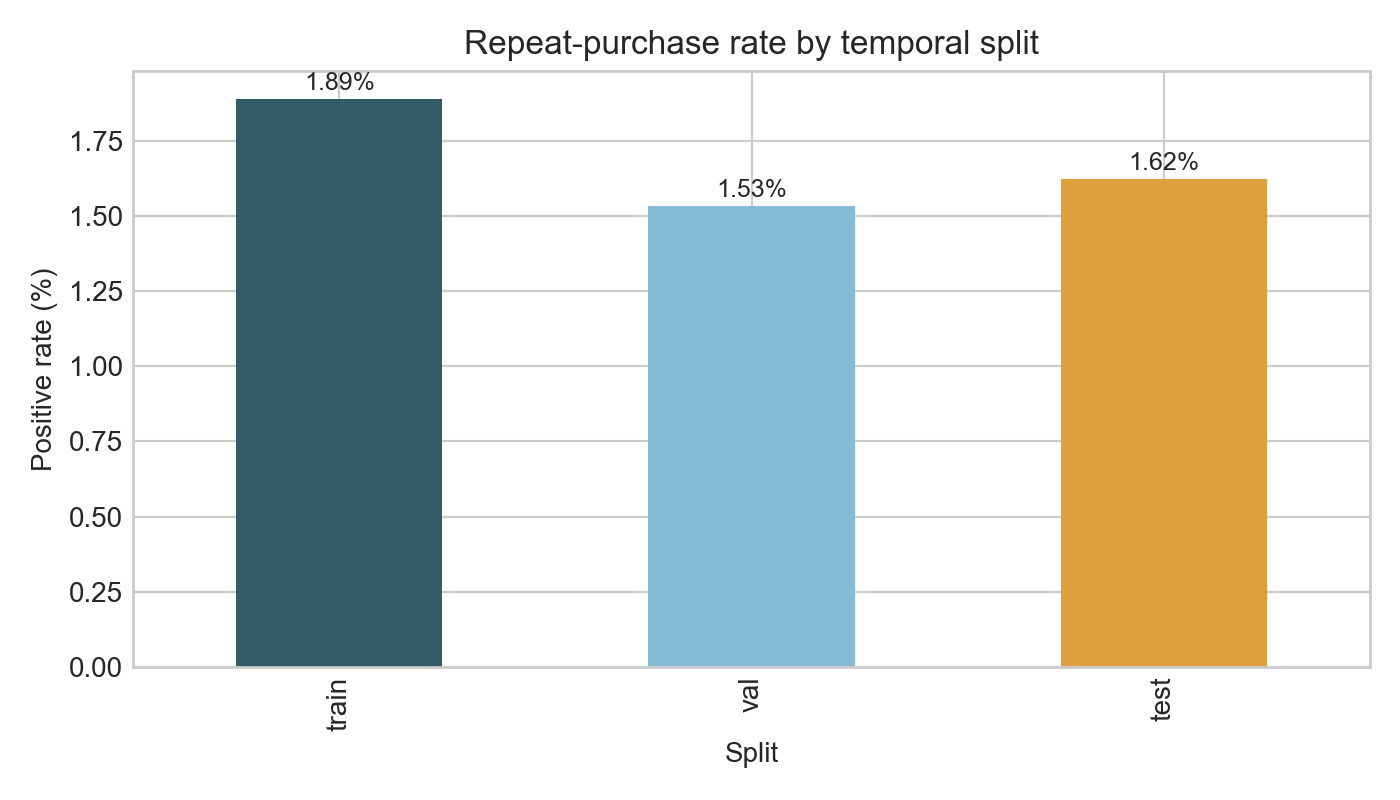
\includegraphics[width=0.7\textwidth]{figures/target_rate_by_split.png}
\caption{Target rate across temporal splits.}
\end{figure}

EDA showed four important properties. First, the task is highly imbalanced, so PR-AUC and Lift@10\% are more meaningful than accuracy. Second, review text is missing for more than half of customers, so text-only models are unlikely to dominate. Third, several monetary and logistics variables are strongly right-skewed, which motivated log transforms. Fourth, the dataset is inherently temporal, so chronological splitting is necessary.

\section{Feature Engineering}
Feature engineering was driven by domain logic rather than arbitrary transformation. The main feature groups were:
\begin{itemize}
\item review features: score, text presence, text length
\item monetary features: total price, freight, payment value, freight ratio, payment gap
\item order complexity: item count, product count, seller count
\item delivery features: approval lag, delivery days, clipped delivery delay
\item geographic context: customer state, seller state, same-state indicator
\item product context: dominant category and package size proxies
\end{itemize}

These features encode the quality and friction of the customer's first-order experience. That is appropriate for repeat-purchase prediction because retention is often shaped by logistics quality, cost burden, and overall order experience.

\section{Methodology}
Phase 1 compares six baseline models:
\begin{enumerate}
\item Dummy prior classifier
\item Review-score logistic regression
\item Tabular logistic regression
\item Tabular random forest
\item Text-only TF-IDF logistic regression
\item Combined TF-IDF plus tabular logistic regression
\end{enumerate}

Thresholds were selected on the validation split by maximizing F1. Final comparison uses PR-AUC, ROC-AUC, Precision@10\%, Lift@10\%, F1, recall, precision, and Brier score.

The final recommended model is the tabular random forest. It is chosen because it is the strongest baseline on held-out PR-AUC while still being easy to explain. It captures nonlinear interactions among freight burden, delivery friction, review quality, and order complexity better than the linear baselines.

\section{Results}
\subsection{Held-Out Test Results}
\begin{table}[H]
\centering
\small
\begin{tabular}{lrrrrrrr}
\toprule
Model & PR-AUC & ROC-AUC & P@10\% & Lift@10\% & F1 & Recall & Brier \\
\midrule
Dummy prior & 0.0162 & 0.5000 & 0.0140 & 0.8666 & 0.0000 & 0.0000 & 0.0160 \\
Review-score LR & 0.0205 & 0.5799 & 0.0255 & 1.5756 & 0.0440 & 0.3780 & 0.2395 \\
Tabular LR & 0.0224 & 0.5886 & 0.0268 & 1.6544 & 0.0396 & 0.2992 & 0.2181 \\
\textbf{Tabular RF} & \textbf{0.0229} & 0.5698 & 0.0255 & 1.5756 & 0.0434 & 0.2913 & 0.0856 \\
Text TF-IDF LR & 0.0169 & 0.4758 & 0.0179 & 1.1029 & 0.0454 & 0.0945 & 0.1475 \\
Combined TF-IDF + LR & 0.0184 & 0.5303 & 0.0192 & 1.1817 & 0.0335 & 0.1260 & 0.1546 \\
\bottomrule
\end{tabular}
\caption{Phase-1 baseline comparison on the held-out test set.}
\end{table}

\begin{figure}[H]
\centering
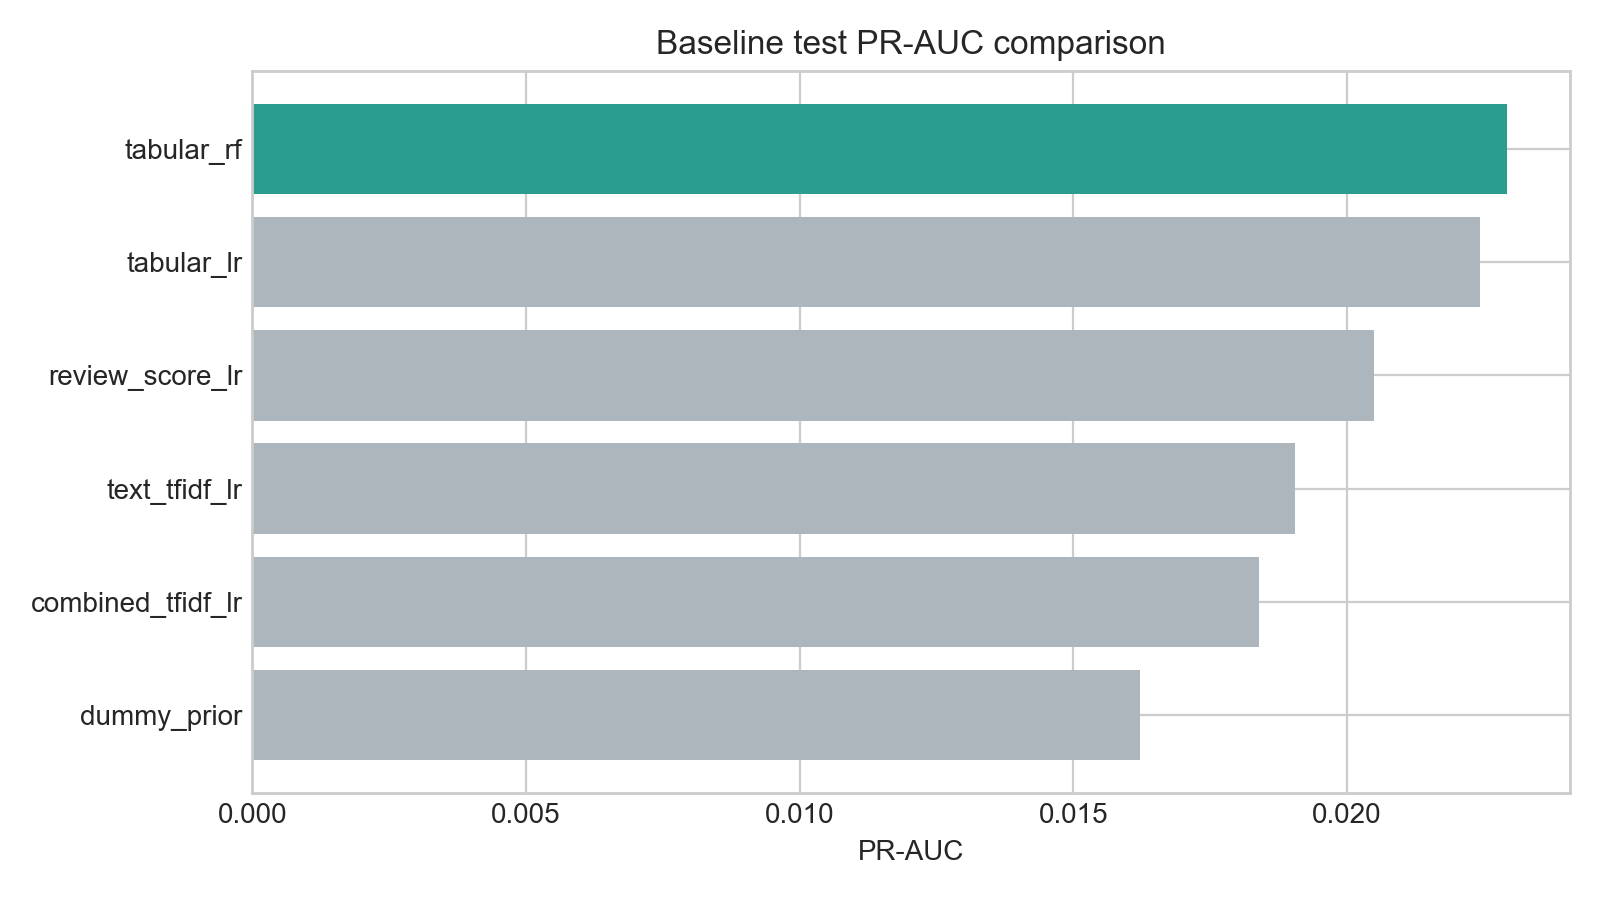
\includegraphics[width=0.9\textwidth]{figures/baseline_test_pr_auc_comparison.png}
\caption{Test PR-AUC across the baseline ladder.}
\end{figure}

\begin{figure}[H]
\centering
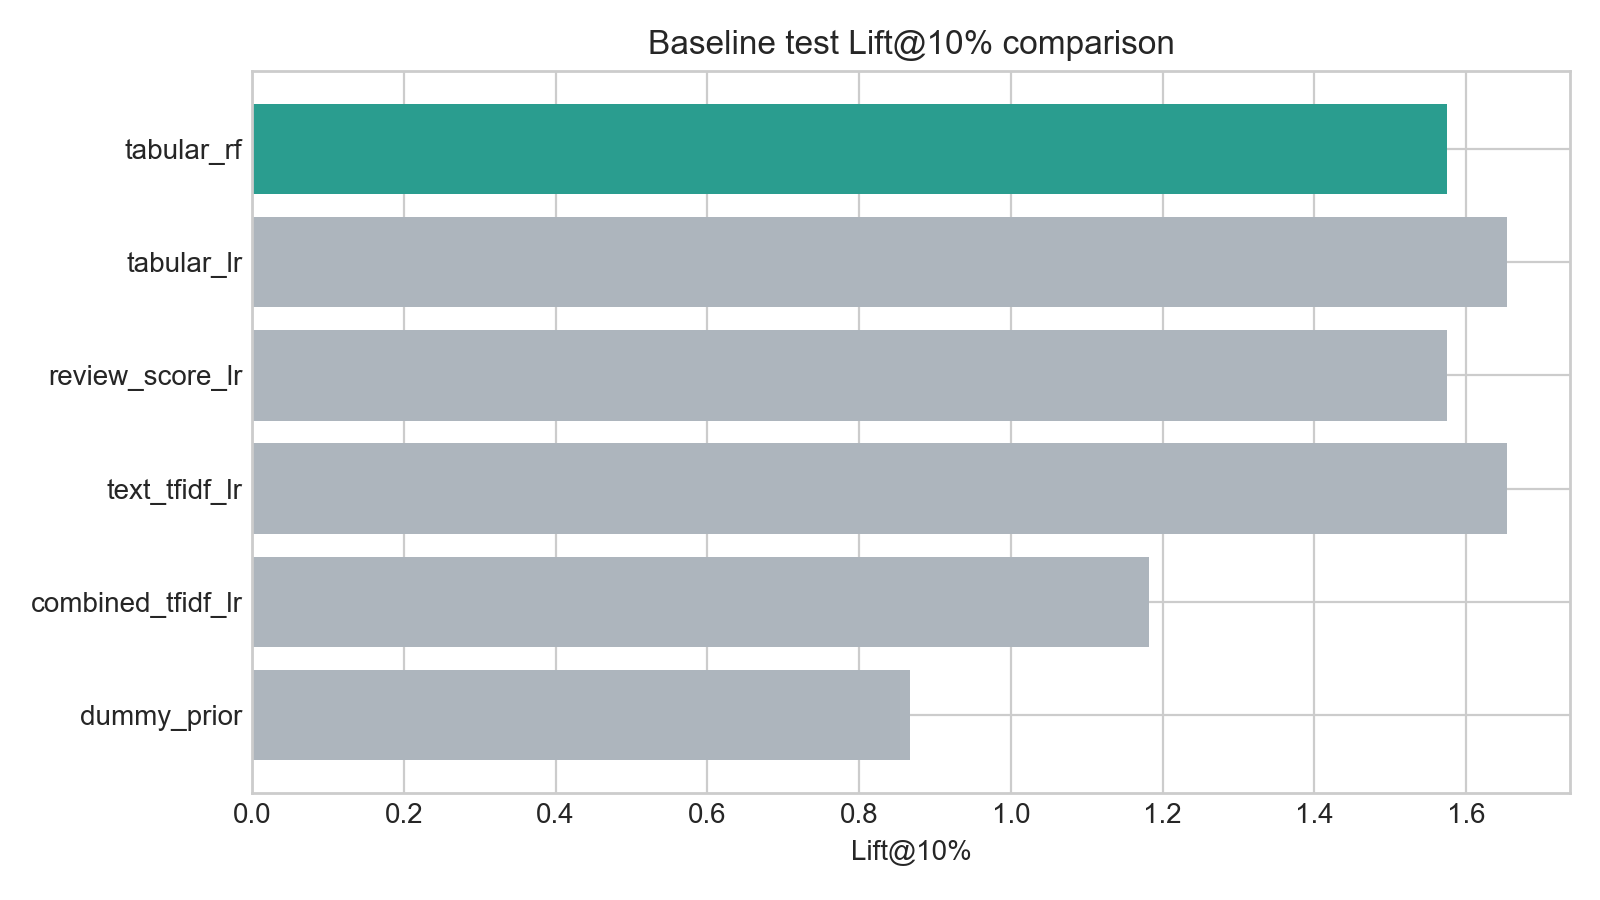
\includegraphics[width=0.9\textwidth]{figures/baseline_test_lift_comparison.png}
\caption{Test Lift@10\% across the baseline ladder.}
\end{figure}

\subsection{Interpretation}
The empirical story is simple. Structured tabular baselines are stronger than text-only baselines. The tabular random forest achieves the best held-out PR-AUC, while tabular logistic regression remains competitive and slightly stronger on ROC-AUC and Precision@10\%. This makes the final recommendation easy to defend: the random forest offers the strongest overall ranking quality among the phase-1 baselines without unnecessary complexity.

Compared with the dummy prior baseline, the final model improves PR-AUC from 0.0162 to 0.0229 and raises Lift@10\% from 0.8666 to 1.5756. This means the top-decile ranked segment contains positives at about 1.58 times the average rate, which is useful for CRM prioritization.

\section{Explainability}
Explainability was applied at three levels:
\begin{itemize}
\item permutation importance for the final tabular random forest
\item partial dependence plots for selected operational features
\item positive and negative text terms from the text logistic model
\end{itemize}

\begin{figure}[H]
\centering
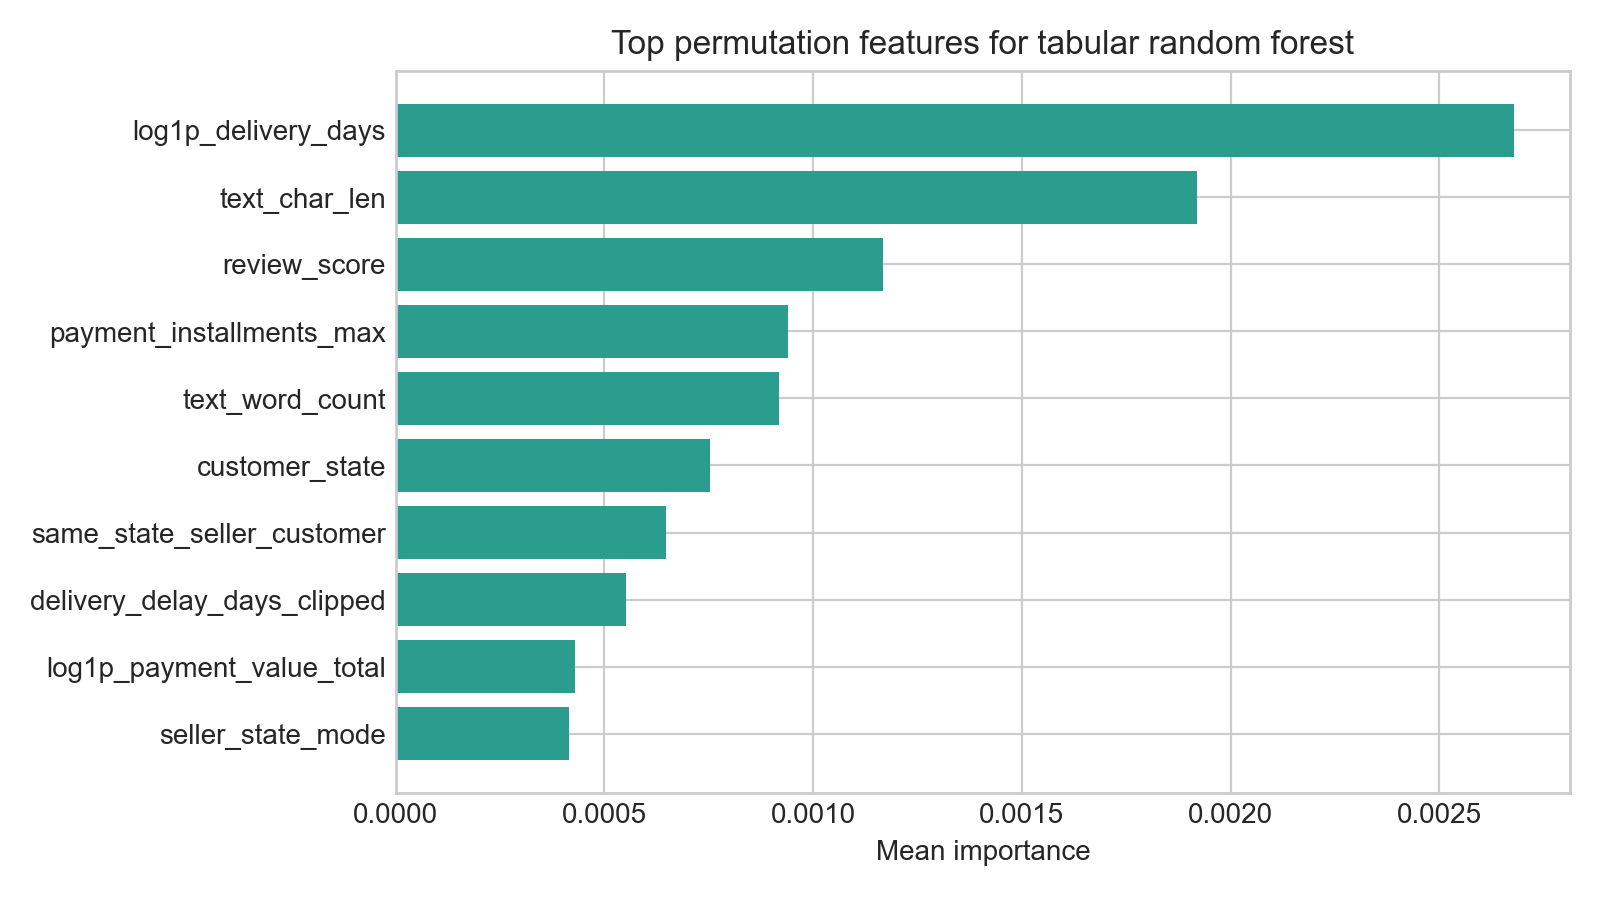
\includegraphics[width=0.9\textwidth]{figures/baseline_top_permutation_features.png}
\caption{Top permutation features for the final phase-1 model.}
\end{figure}

The most important features are operational and business-facing: review score, freight burden, delivery timing, item count, payment value, and text-length proxy variables. These features align with intuition: better first-order experience and lower operational friction support repeat purchase.

\section{Theoretical Discussion}
This project connects core theory to observed results. Class imbalance makes PR-AUC more appropriate than accuracy. Temporal dependence motivates chronological splitting instead of random splitting. Sparse and highly missing review text limits the ceiling for text-only models. The bias-variance tradeoff also appears clearly: linear models are transparent and stable, while random forest captures nonlinear effects that improve ranking quality.

\section{Failure Analysis and Limitations}
This phase-1 system has realistic limitations:
\begin{itemize}
\item the target event is rare, so absolute PR-AUC remains modest
\item review text is missing for a large share of customers
\item Portuguese text reduces interpretability for non-Portuguese readers
\item the model is optimized for ranking rather than perfect classification
\end{itemize}

The main failure pattern is also interpretable. When two customers have similar structured business profiles, sparse review text usually does not add enough signal to change ranking materially. That is why the text-only and combined linear models remain weaker than the strongest tabular baseline.

\section{Conclusion}
This project delivers a complete and leakage-safe phase-1 predictive analytics system for repeat-purchase prediction. The recommended final model is the tabular random forest baseline. The central finding is that structured first-order business signals are more predictive than sparse review text for this retention task, while text remains useful for interpretation.

\begin{thebibliography}{9}
\bibitem{olist}
Olist. \emph{Brazilian E-Commerce Public Dataset by Olist}. Kaggle dataset release.

\bibitem{salton1988}
G. Salton and C. Buckley.
\newblock Term-weighting approaches in automatic text retrieval.
\newblock \emph{Information Processing and Management}, 24(5):513--523, 1988.

\bibitem{breiman2001}
L. Breiman.
\newblock Random forests.
\newblock \emph{Machine Learning}, 45(1):5--32, 2001.

\bibitem{molnar2022}
C. Molnar.
\newblock \emph{Interpretable Machine Learning}.
\newblock 2nd edition, 2022.
\end{thebibliography}

\end{document}
